\documentclass{article}
\usepackage[letterpaper,body={6.3in,9.15in},top=.8in,left=1.1in]{geometry}
\usepackage{fancyvrb,color,gretl}
\usepackage{amsmath}
\usepackage{graphicx}
\usepackage[authoryear]{natbib}
\usepackage[pdftex,hyperfootnotes=false]{hyperref}

\definecolor{steel}{rgb}{0.03,0.20,0.45}

\hypersetup{pdftitle={gretl regls},
            pdfauthor={Allin Cottrell},
            colorlinks=true,
            linkcolor=blue,
            urlcolor=red,
            citecolor=steel,
            bookmarksnumbered=true,
            plainpages=false
          }

\setlength{\parskip}{1ex}
\setlength{\parindent}{0pt}
\setcounter{secnumdepth}{1}
\setcounter{tocdepth}{1}

\renewcommand{\floatpagefraction}{.8}

\newcommand{\startappendices}{%
\newcounter{appcount}
\setcounter{appcount}{0}
\renewcommand{\thesection}{Appendix \Alph{appcount}}}

\newcommand{\myappendix}[1]{%
\addtocounter{appcount}{1}
\section{#1}}

\newenvironment{funcdoc}
{\noindent\hrulefill\\[-12pt]}
{\medbreak}

\title{\textsf{regls}: regularized least squares for gretl}
\author{Allin Cottrell}
\date{April 29, 2024}

\begin{document}
\maketitle

\section{Introduction}
\label{sec:intro}

The \textsf{regls} addon is essentially a front-end for functionality
coded in C in the gretl \texttt{regls} plugin; to run the package you
will need gretl version 2020e or higher.  The plugin implements LASSO
\citep{tibshirani96}---by default via the Alternating Direction Method
of Multipliers (ADMM) algorithm as set out in \cite{boyd2010}; Ridge
regression, by default via Singular Value Decomposition; and the
``elastic net'' hybrid of LASSO and Ridge.

The best-known implementation of regularized regression is that
provided by the \textsf{glmnet} package for \textsf{R}. Since we make
several references to \textsf{glmnet} below we should state up front
what we're talking about. The authors of \textsf{glmnet} are Jerome
Friedman, Trevor Hastie, Rob Tibshirani, \textit{et al}.  Current
information on \textsf{glmnet} can be found at
\url{https://glmnet.stanford.edu/}; for further information on the
algorithms used in the package see \cite{glmnet10}.\footnote{We should
  point out that \textsf{glmnet} supports regularized estimation of
  generalized linear models. At present \textsf{regls} only supports
  least squares.}

This package supports LASSO, Ridge and elastic net via the functions
\texttt{regls()} and \texttt{mregls()}. The first of these requires
that a dataset is in place while the second accepts data in matrix
form, otherwise they are essentially the same; see
Section~\ref{sec:funcref} for details on \texttt{mregls()}.  We begin
by discussing LASSO, which is the default method.  Ridge is discussed
in Section~\ref{sec:ridge} and elastic net in Section~\ref{sec:elnet}.

We use the LASSO parameterization employed by Boyd \textit{et al}: the
objective is
\begin{equation}
  \label{eq:obj}
  \min_{\hat{\beta}} \quad \frac{1}{2}\,
  \sum_{i=1}^n (y_i - X_i\hat{\beta})^2 + \lambda \sum_{j=1}^k |\hat{\beta}_j|
\end{equation}
where $n$ is the number of observations, $k$ is the number of
candidate regressors (the number of columns of $X$) and
$\lambda \geq 0$ is the LASSO regularization hyperparameter. In this
context $\lambda = 0$ gives plain OLS, and at the other end of the
spectrum there exists a data-dependent value of $\lambda$, namely
\begin{equation}
  \label{eq:lmax}
  \lambda_{\max} = \|X'y\|_{\infty}
\end{equation}
which drives all elements of $\hat{\beta}$ to zero.  A key control
variable for our \texttt{regls} function is the scaled term
$s = \lambda/\lambda_{\max}$, such that $0 \leq s \leq 1$.

The \texttt{regls} function takes three arguments: a series (the
dependent variable), a list (the independent variables, not including
a constant) and a bundle to contain optional parameters; and it
returns a bundle, described below. Its signature is therefore
\begin{code}
function bundle regls (series y, list X, bundle parms)
\end{code}

The \texttt{parms} argument may be omitted, in which case all settings
assume their default values, described below.

\section{Basic options}
\label{sec:basic-opts}

One basic element in the \texttt{parms} bundle is a specification for
$\lambda$, which may take either of two forms, as follows:
\begin{enumerate}
\item under the key \texttt{lfrac} (``lambda fraction''), a scalar
  (single $s$ value) or vector (sequence of $s$ values); or
\item under the key \texttt{nlambda}, the number of $s$ values to be
  used ($\geq 4$), in which case the values will be assigned
  automatically.
\end{enumerate}
If \texttt{nlambda} is provided instead of \texttt{lfrac}, the
automatic $s$ vector is a declining logarithmic sequence starting at 1
and finishing at 0.0001. For example, given \texttt{nlambda} = 5 the
sequence will be $s$ = \{1, 0.1, 0.01, 0.001, 0.0001\}.

If neither \texttt{lfrac} nor \texttt{nlambda} is specified, the
default is as if \texttt{nlambda} were given as 25.

In case you wish to specify a sequence succinctly but with more
control, the package contains a utility function
\texttt{lambda\_sequence()}, which takes up to three arguments. The
first and second arguments (required) give the maximum $s$ and the
number of values, while the third (optional) argument can be used to
give the minimum $s$ (by default 0.0001). As with the \texttt{nlambda}
option the values are spaced logarithmically.  So if you were to do
\begin{code}
parms.lfrac = lambda_sequence(1, 20, 0.001)
\end{code}
the resulting sequence would be $s$ = \{1, 0.69519, 0.48329, \dots,
0.00144, 0.001\}.

To be clear, if no option pertaining to $\lambda$ is given that's
equivalent to
\begin{code}
parms.lfrac = lambda_sequence(1, 25, 0.0001)
\end{code}
while if \texttt{nlambda = 100} is given that's equivalent to
\begin{code}
parms.lfrac = lambda_sequence(1, 100, 0.0001)
\end{code}

A second basic member of the parameter bundle is \texttt{stdize}, a
boolean switch to toggle standardization of the data. The default is
to perform standardization (corresponding to a non-zero value of this
option), but if the data are already standardized on input
\texttt{stdize} may be set to 0.  The estimates include an intercept
(which is not subject to regularization) only if \texttt{stdize} is
on.

Another basic option is \texttt{verbosity}. This has a default value
of 1, meaning that \texttt{regls} prints out a certain amount of
information about its progress and/or results. Setting it to 0 makes
\texttt{regls} run (mostly) quietly; setting it to 2 or 3 produces
more output in some cases.

The further optional parameters, as well as the contents of the bundle
returned by \texttt{regls}, are best explained by reference to the
various modes of usage of the function, namely estimation with a
single value of $\lambda$; exploration of a range of $\lambda$ values
using a unified training sample; and (probably most relevant in
practice) search for optimal $\lambda$ via cross validation. For
reference, the script in Listing~\ref{script:123} illustrates
basic usage for each of these modes.

\begin{script}[htbp]
  \caption{Basic LASSO examples}
  \label{script:123}
\begin{scode}
set verbose off
clear --all
include regls.gfn

# Use the supplied data on crime-rates by locality
open murder.gdt --quiet --frompkg=regls

# The dependent variable will be the murder rate, and we
# select 101 candidate regressors with no missing values
series y = murdPerPop
list X = population..LemasPctOfficDrugUn

# set training sample range
smpl 1 1000

# select a case to run
CASE = 1 # or 2, or 3

if CASE == 1
   # single regularization
   bundle b = regls(y, X, _(lfrac = 0.5))
elif CASE == 2
   # multiple lambdas, no cross validation
   bundle b = regls(y, X, _(nlambda=50))
else
   # multiple lambdas with cross validation
   bundle parms = _(nlambda=50, xvalidate=1, nfolds=10)
   bundle b = regls(y, X, parms)
endif

# set testing sample range
smpl 1001 1200

# take a look at basic out-of-sample stats
series yhat = regls_pred(b, X)
matrix s = regls_get_stats(y, yhat)
print s
\end{scode}
\end{script}

\section{Estimation with a single regularization}
\label{sec:single-lambda}

Suppose we have 1200 observations on some series \texttt{y} and list
\texttt{X} (with $k=100$ members) and we wish to train on the first
1000 observations, using $s = 0.2$, then predict for the remaining
200. And let's say the data are not pre-standardized. We might then
do:
\begin{code}
bundle parms = _(lfrac = 0.2)
smpl 1 1000
bundle b = regls(y, X, parms)
\end{code}
We'll then find the following in \texttt{b}:
\begin{itemize}
\item \texttt{B}: The full vector of $k+1$ coefficients, including an
  intercept---unless \texttt{stdize} is set to 0 in which case
  \texttt{B} will have $k$ elements.
\item \texttt{nzb}: A vector holding only the non-zero coefficients.
\item \texttt{nzX}: A list identifying the regressors with non-zero
  coefficients.
\item \texttt{lmax}: The $\lambda_{\max}$ value for the standardized
  data.
\item \texttt{lambda}: The value of $\lambda = s\,\lambda_{\max}$, see
  (\ref{eq:lmax}) above.
\item \texttt{crit}: The minimized LASSO criterion, see (\ref{eq:obj})
  above.
\item \texttt{R2}: Coefficient of determination,
  $1 - \sum(y-\hat{y})^2/\sum(y-\bar{y})^2$.
\item \texttt{BIC}: The Bayesian Information Criterion for the
  estimated model.
\item \texttt{nobs}: The number of training observations used.
\item \texttt{lfrac}: The input value of $s$.
\item \texttt{stdize}: Whether \texttt{regls} did standardization or
  not.
\end{itemize}

At some points below we refer to the coefficient of determination
(under the key \texttt{R2}) as ``$R^2$''. But note that with
regularized regression, unlike OLS, this figure is not equal to the
squared correlation between $y$ and $\hat{y}$.

\section{Exploring a range of regularizations}
\label{sec:simple-search}

Suppose we wish to compare results from ten values of $\lambda$,
using all the training data. We might then revise the prior script as:
\begin{code}
bundle parm = _(nlambda = 10)
smpl 1 1000
bundle b = regls(y, X, parms)
\end{code}

In this case \texttt{b.B} will be a matrix holding the full
coefficient vector for each $s$ (one column per $s$ value); and
\texttt{b.crit}, \texttt{R2} and \texttt{b.BIC} will be column
vectors of length 10 holding LASSO criterion, $R^2$ and BIC for each
$s$, respectively. In addition the bundle will contain:
\begin{itemize}
\item \texttt{lfmin}: The $s$ value which produces the smallest BIC
  value.
\item \texttt{idxmin}: The 1-based index of \texttt{lfmin} in the
  vector of $\lambda$ values.
\end{itemize}

The BIC \citep{schwarz78} is calculated by \textsf{regls} as
$-2\ell(\hat{\beta}) + k^*(\lambda) \log n$, where $\ell(\hat{\beta})$
is the log-likelihood, based on the sum of squared residuals, and
$k^*(\lambda)$ the number of non-zero coefficients for the given
$\lambda$. This criterion provides a guide (though certainly not an
infallible one) to the likely out-of-sample performance of a model:
smaller values of BIC are better. Note that the LASSO criterion itself
does not offer such a guide (it is likely to decrease monotonically
along with $\lambda$), but it can be useful in comparing the
effectiveness of minimization algorithms (see \ref{app:ccd}).

When multiple $\lambda$ values are specified, the vector \texttt{nzb}
and list \texttt{nzX} refer to the non-zero coefficients and
associated regressors obtained with $s$ = \texttt{lfmin} (the BIC
minimizer).

\section{Optimizing via cross validation}
\label{sec:xvalid}

Searching for optimal $\lambda$ over the entire training sample we run
the risk of overfitting. The standard remedy is to divide the training
data into ``folds'' and do cross validation. The algorithm is then (in
pseudo-code):
\begin{code}
for each s value, s(j)
  MSE(j) = 0
end
for each fold, f(i)
  set the estimation sample to the complement of f(i)
  for each s value, s(j)
    perform regularized estimation using s(j) and predict for f(i)
    MSE(j) <- MSE(j) + MSE for f(i)
  end
end
\end{code}
We then perform regularized estimation on the full training data using the
$s$ value that yields the least total MSE on the above procedure (or
perhaps take an alternative approach---see below).

The options connected with cross validation (to be entered in the
parameter bundle passed to \texttt{regls}) are as follows:
\begin{itemize}
\item \texttt{xvalidate}: Boolean, trigger for doing cross validation (required).
\item \texttt{nfolds}: Integer, the number of folds (optional, default
  10).
\item \texttt{randfolds}: Boolean, whether the folds should be
  assigned randomly (optional, default 0).
\item \texttt{seed}: Integer, relevant only when \texttt{randfolds} is
  selected. By setting a specific seed for the random-number generator
  you can get exactly repeatable results.
\end{itemize}

At present the folds are either assigned at random or (by default)
they are sequences of consecutive observations. It may be worth adding
a facility to set the folds via a predefined series. A further point:
at present the folds are by construction all the same size---the
result of integer division of the number of training observations by
the number of folds, which means that any ``remainder'' training
observations are ignored. That could be generalized if it seems
worthwhile.

When cross validation is specified \texttt{regls} will print some
information on the performance of the values of $s$ used, a
snippet of which is shown below:
\begin{code}
          s        MSE         se
   1.000000   1.000000   0.063336
   0.615848   0.870633   0.057432
   0.379269   0.759641   0.048581
   0.233572   0.694237   0.043515
\end{code}
%
The \texttt{MSE} value is the mean across the folds, and \texttt{se}
is its standard error, computed as per \textsf{glmnet}.  The
\texttt{crit} member of the returned bundle is then a two-column
matrix, holding the mean MSE values (in column 1) and their standard
errors (in column 2).

While it would seem most natural to select for prediction the $s$
value that minimizes MSE on cross validation---call this
$s^*$---\textsf{glmnet} suggests an alternative policy: select the
largest $s$ that delivers an MSE within one standard error of the
minimum, which we'll call $s^{\dagger}$. It may be that $s^*$ and
$s^{\dagger}$ are the same value, but if not this policy gives the
benefit of the doubt to parsimony.

After cross validation, the bundle returned by \texttt{regls} contains
the full coefficient matrix (one column per value of $s$), estimated
on the full training data, under the key \texttt{B}.  It also holds
the indices of both $s^*$ and $s^{\dagger}$, under the keys
\texttt{idxmin} and \texttt{idx1se} respectively.

\section{Obtaining predicted values}
\label{sec:predict}

Optimization of out-of-sample prediction is of course the name of the
game with regularized regression. To obtain out-of-sample predictions
(and/or within-sample fitted values if you want them), the recommended
approach is to use \texttt{regls\_pred()}. This function takes two
arguments: a bundle produced by \texttt{regls()} and the list passed
to \texttt{regls} as \texttt{X}. By default the return value is a
series holding predicted values.

If you use \texttt{mregls()} for estimation, the alternative
prediction function \texttt{mregls\_pred()} should be called in place
of \texttt{regls\_pred}. In that case the second argument should be a
matrix of regressors with the same number of columns as that passed to
\texttt{mregls}, and by default the return value is a column vector of
length equal to the row dimension of the matrix argument.

In each case the default predictions are based on either the unique
coefficient vector if just one value of $\lambda$ was used, or the
``preferred'' coefficient vector in the case of multiple $\lambda$
values---that is, the BIC minimizer if cross-validation is not
performed, or that corresponding to either \texttt{idxmin} or
\texttt{idx1se} (see above) after cross-validation. The
\texttt{idxmin} value is used automatically unless \texttt{use\_1se}
was set in the parameter bundle passed to \texttt{regls} or
\texttt{mregls}.

\subsection{An example}

Suppose, for example, that the available data comprise 1200
observations, the first 1000 of which were used for training and 200
of which remain for testing. And suppose that a bundle named
\texttt{b} has been obtained via \texttt{regls} using a list of
regressors \texttt{X}. Then the following would serve to obtain
predictions under the name \texttt{yhat} for the testing observations:
\begin{code}
smpl 1001 1200
series yhat = regls_pred(b, X)
\end{code}
The case of matrix data is similar, except that the \texttt{smpl}
command is not relevant. If you have an \texttt{X} matrix of 1200 rows
you might pass \texttt{X[1:1000,]} to \texttt{mregls}, then predict
for the remainder of the observations via
\begin{code}
matrix yhat = mregls_pred(b, X[1001:,])
\end{code}

\subsection{Further options}

Beyond the default behavior of the prediction functions, if multiple
$\lambda$ values were used in estimation you can control the output by
adding a preference to the bundle \texttt{b}, under the key
\texttt{pred}, before passing it to \texttt{regls\_pred} or
\texttt{mregls\_pred}. The admissible values for \texttt{pred} are as
follows:
\begin{enumerate}
\item \texttt{idxmin}: use the \texttt{idxmin} column of the \texttt{B}
  coefficient matrix for prediction (after cross validation only).
\item \texttt{idx1se}: use the \texttt{idx1se} column of \texttt{B}
  for prediction (after cross validation only).
\item A scalar value between 1 and the number of $\lambda$ values, to
  select a specific column from \texttt{B}.
\item A row vector to select multiple columns from
  \texttt{B}.\label{p:sel}
\item The keyword \texttt{all} to produce predictions from all columns of
  \texttt{B}.\label{p:all}
\end{enumerate}

Note that if alternatives~\ref{p:sel} or \ref{p:all} are used, output
takes the form of a matrix, even if estimation was by
\texttt{regls}. The \texttt{mat2list()} built-in function can create a
list of series from such a matrix if you want.

\subsection{Manual prediction}

You can generate predictions yourself using built-in functionality,
such as the \texttt{lincomb()} function or matrix multiplication,
applied to elements of the bundle obtained from estimation. But note
that if \texttt{regls} or \texttt{mregls} performs standardization the
first row of \texttt{B} will hold an estimated intercept for each
$\lambda$. This does not match an entry in the regular list or matrix
of regressors, \texttt{X}, but must be taken into account. For
example, if you wish to predict manually using an arbitrary column,
\texttt{j}, of \texttt{B} after \texttt{regls} you can do
\begin{code}
list All = const X
series fitted = lincomb(All, b.B[,j])
\end{code}
This sort of thing is handled automatically by the specialized
prediction functions described above.

\section{Execution speed}
\label{sec:speed}

According to the discussion in Section 3.2.2 of \cite{boyd2010}: the
ADMM algorithm is reliable but is known \textit{not} to be fast (or
not if accurate results are wanted). However, we have been able to
accelerate ADMM to the point where execution time is unlikely to be an
issue, by two main means.
\begin{itemize}
\item We implemented the suggestion in Section 3.4.1 of
  \cite{boyd2010}: letting the penalty factor $\rho$ vary across ADMM
  iterations to keep the magnitudes of the primary and dual residuals
  in rough balance. This turns out to be highly effective.
\item We implemented automatic ``farming out'' of cross validation to
  multiple \textsf{MPI} processes (when \textsf{MPI} is available on
  the host machine). It's possible to prevent this by adding
  \texttt{no\_mpi} to the parameter bundle with a non-zero value.
\end{itemize}
In one benchmark case we considered---with 1500 training observations,
101 covariates, 50 values of $\lambda$ and 10 randomized cross
validation folds---the execution time was about 13 seconds before
making the changes mentioned above, and about 1.5 seconds
thereafter.\footnote{On a desktop machine with 4 Intel i7 processors,
  running Linux.}

\section{Additional ADMM controls}
\label{sec:add-controls}

This section describes some additional controls over the ADMM
algorithm that can be passed to the \texttt{regls} function via the
\texttt{parms} bundle. Under the key \texttt{admmctrl} you can supply
a 3-vector whose elements are, in order:
\begin{itemize}
\item \texttt{rho}: a positive real number, the initial ADMM penalty
  parameter. It seems that $\rho = 8.0$ works well but higher or lower
  values might produce faster convergence in some cases.
\item \texttt{reltol}: the relative tolerance used in gauging whether
  the algorithm has converged sufficiently.
\item \texttt{abstol}: the absolute convergence tolerance (which will
  be scaled by the square root of the number of candidate regressors).
\end{itemize}
We have found that \texttt{reltol} and \texttt{abstol} values of
$10^{-4}$ and $10^{-6}$, respectively, produce reasonably accurate
results in a manageable number of iterations. Setting smaller values
will produce greater accuracy at the cost of more iterations.
Non-positive values of these terms are ignored, so one can, for
example, set a single element by passing a zero vector with just the
desired term set to a positive value.

\section{LASSO examples}
\label{sec:examples}

Besides the sample script supplied with the package, more examples can
be found in the directories \texttt{murder}, \texttt{wine} and
\texttt{fat} at \url{http://gretl.sourceforge.net/lasso/}.  Some of
these scripts incorporate comparison with \textsf{glmnet}.  The
murder-rate and wine quality examples use real-world data; the
\texttt{fat} example is an artificial case with more regressors than
observations.

Note that it's necessary to run the scripts involving randomized cross
validation several times to get a good idea of what's going on: in
each case there seem to be a few ``favored solutions'' of varying
probability. Sometimes one sees \textsf{regls} finding the better one,
sometimes \textsf{glmnet}.

\section{Ridge regression}
\label{sec:ridge}

While LASSO involves $\ell_1$ regularization, Ridge uses $\ell_2$: the
penalty factor $\lambda$ applies to the sum of squared coefficients,
giving rise to the following objective:
\begin{equation}
  \label{eq:ridge-obj}
  \min_{\hat{\beta}} \quad
  \sum_{i=1}^n (y_i - X_i\hat{\beta})^2 + \lambda \sum_{j=1}^k \hat{\beta}_j^2
\end{equation}

In consequence, although a large value of $\lambda$ will shrink Ridge
estimates substantially relative to OLS it will not send any
coefficients to exactly zero as does LASSO. If the $X$ matrix exhibits
strong collinearity, LASSO will tend to eliminate most of the
collinear terms while Ridge will tend to distribute the predictive
weight across the terms, yielding several small coefficients instead
of one relatively substantial coefficient and a bunch of zeros.

To get the \texttt{regls} function to perform Ridge regression rather
than LASSO, set a value of 1 under the key \texttt{ridge} in the
\texttt{parms} bundle, as in
\begin{code}
parms.ridge = 1
\end{code}

Most of the points made above with respect to LASSO carry over to
Ridge. The same three modes of operation described in Sections
\ref{sec:single-lambda} to \ref{sec:xvalid} (from estimation using a
single value of $\lambda$ to cross-validation with as many values as
you like) are available.

There is an important difference, however, in respect of the
calibration of $\lambda$. In the LASSO case there's an easily computed
$\lambda_{\max}$ (= $\|X'y\|_{\infty}$) which just suffices to force
all slope coefficients to zero and so, as explained above, the user is
asked to express the LASSO penalty as a fraction of this maximum. In
the case of Ridge there is generally no finite $\lambda$ that will
drive all coefficients to zero and so no ``natural'' maximum to serve
as a benchmark. We therefore offer the user three options for the
specification of ``\texttt{lfrac},'' controlled by the integer-valued
parameter \texttt{lambda\_scale}:
\begin{itemize}
\item \texttt{lambda\_scale} = 0: no scaling is performed. The
  ``\texttt{lfrac}'' values are taken as actual $\lambda$ values (and
  so do not have to be bounded by 1.0 above).
\item \texttt{lambda\_scale} = 1 (the default): we emulate
  \textsf{glmnet}. The largest value of $\lambda$ is set to
  $9.9 \times 10^{35}$, which will drive all coefficients to
  near-zero. The second-largest $\lambda$ (call it $\lambda_2$) is
  then set to 1000 times $\|X'y\|_{\infty}$, and subsequent values in
  the sequence are scaled in relation to $\lambda_2$.
\item \texttt{lambda\_scale} = 2: we follow the suggestion of some
  practitioners, setting $\lambda_{\max}$ to the squared Frobenius
  norm of $X$, which will not drive all coefficients to near-zero but
  will impose substantial shrinkage in relation to OLS.
\end{itemize}

To be clear on the action of options 1 and 2 for
\texttt{lambda\_scale}, suppose our \texttt{lfrac} specification is
\begin{code}
lfrac = {1, 0.5, 0.25, 0.125}
\end{code}
Then if \texttt{lambda\_scale} = 1 this translates to
\begin{code}
lam2 = 1000 * infnorm(X'y)
effective_lambda = {9.9e35, lam2, 0.5*lam2, 0.25*lam2}
\end{code}
while if \texttt{lambda\_scale} = 2 it becomes
\begin{code}
lam1 = tr(X'X) # Frobenius norm squared
effective_lambda = {lam1, 0.5*lam1, 0.25*lam1, 0.125*lam1}
\end{code}
Note that the relevant matrix norms are computed after
standardization.

One further point on the scaling of $\lambda$: since the key
\texttt{lfrac} doesn't look right when \texttt{lambda\_scale} = 0, we
accept \texttt{lambda} as an alternative key. In fact, if
\texttt{lambda} rather than \texttt{lfrac} is found in the input
bundle, the default for \texttt{lambda\_scale} switches to 0 (but an
explicit setting will override this).

In addition to \texttt{BIC} and \texttt{R2} the return bundle from
Ridge regression contains \texttt{edf} (a scalar if a single $\lambda$
is specified, otherwise a column vector). This is the ``effective''
degrees of freedom, or number of free parameters, calculated via
the SVD of the matrix of regressors:
\begin{equation}
  \label{eq:edf}
\mbox{edf} = \sum_{i=1}^k\, \frac{\sigma_i^2}{\sigma_i^2 + \lambda}
\end{equation}
where the $\sigma_i$s are the singular values. As a measure of the
``size'' of a model this takes the place of the number of non-zero
coefficients in LASSO.

In the case of a single $\lambda$, when estimation is performed using
the default SVD method, further information is available: the return
bundle contains the covariance matrix of the parameter estimates
(other than the constant) under the key \texttt{vcv}. And if the
\texttt{verbosity} option is set to 2 you get a printout of the model,
showing standard errors, $z$ statistics and $P$-values.

\section{The CCD option}
\label{sec:ccd}

As stated above, the default algorithms used by \textsf{regls} for
LASSO and Ridge are ADMM and SVD, respectively. However, you have the
option---for both LASSO and Ridge---of using the Cyclical Coordinate
Descent (CCD) algorithm, as employed by \textsf{glmnet}. This is
governed by two additional keys in the \texttt{parms} bundle:
\begin{itemize}
\item \texttt{ccd}: boolean, default 0. Set this to 1 to use CCD.
\item \texttt{ccd\_toler}: a positive scalar setting the convergence
  tolerance for CCD. The default is $10^{-7}$ (as in \textsf{glmnet});
  setting a smaller value will give greater accuracy at the expense of
  more iterations.
\end{itemize}

Using CCD will give results that are more directly comparable with
\textsf{glmnet}. Beyond that, practitioners are likely to ask, how do
the algorithms compare in terms of speed and accuracy? This question
is addressed in detail in \ref{app:ccd}. The short answer
is that CCD at its default tolerance is faster but somewhat less
accurate than ADMM and SVD. By tightening the CCD tolerance one can
generally close the accuracy gap; this may or may not reverse the
ranking in terms of speed.

\section{Elastic net}
\label{sec:elnet}

As mentioned above, elastic net is a hybrid of LASSO and Ridge. It
employs a combination of $\ell_1$ and $\ell_2$ penalties governed by a
hyperparameter $0 \leq \alpha \leq 1$. The objective is
\[
    \min_{\hat{\beta}} \quad \frac{1}{2}\,
    \sum_{i=1}^n (y_i - X_i\hat{\beta})^2 +
    \lambda \left(\frac{1-\alpha}{2} \sum_{j=1}^k \hat{\beta}_j^2
      + \alpha \sum_{j=1}^k |\hat{\beta}_j|\right)
  \]
Thus $\alpha = 1$ gives LASSO, $\alpha = 0$ gives Ridge, and anything
between gives a combination. It has been argued that better
out-of-sample prediction can be obtained in some cases by preserving
some highly collinear regressors \`a la Ridge, while sending some
coefficients to exact zero as in LASSO, and elastic net allows for
this.

In the \texttt{regls} function, elastic net is selected by specifying
a fractional value under the key \texttt{alpha} in the parameters
bundle. This automatically switches to the CCD algorithm
(Section~\ref{sec:ccd}), so the \texttt{ccd\_toler} option becomes
applicable.\footnote{In principle the ADMM algorithm could handle
  elastic net, but to date we have not implemented such support.}

When elastic net is used on a sequence of $\lambda$s without cross
validation (see Section~\ref{sec:simple-search}) \texttt{regls}
provides a BIC measure as a possible means of selecting the most
promising penalty factor. This requires calculation of the effective
number of parameters (degrees of freedom), for which we use the method
specified in \cite{zou-hastie05}.

Note that if cross validation is called for with elastic net, it is
only the $\lambda$ value that is optimized. To assess the efficacy of
various $\alpha$ values one would have to perform several cross
validation runs.

\section{GUI usage}

You can access \texttt{regls} in the gretl GUI via the menu item
\textsf{Model/Other linear models/Regularized least squares}. This
brings up the dialog box shown on the left in
Figure~\ref{fig:regls-combo}. Multiple $\lambda$ values and cross
validation are supported as shown. Clicking the \textsf{Advanced}
button gives access to most of the additional options discussed above
(e.g.\ choice of algorithm, seed for randomized cross-validation
folds).

\vspace{1ex}

\begin{figure}[htbp]
  \centering
  \begin{tabular}{cc}
    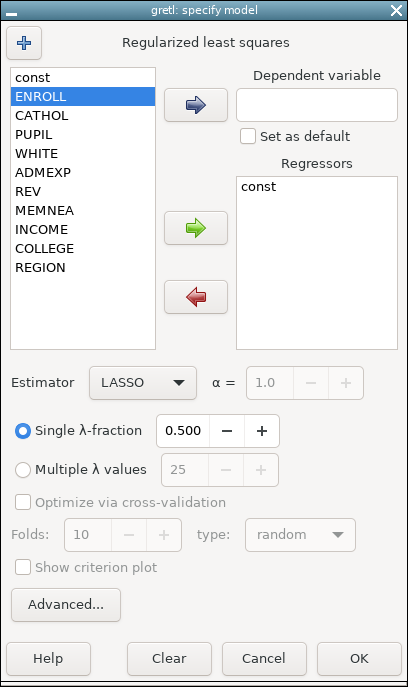
\includegraphics[scale=0.5]{regls_gui} &
    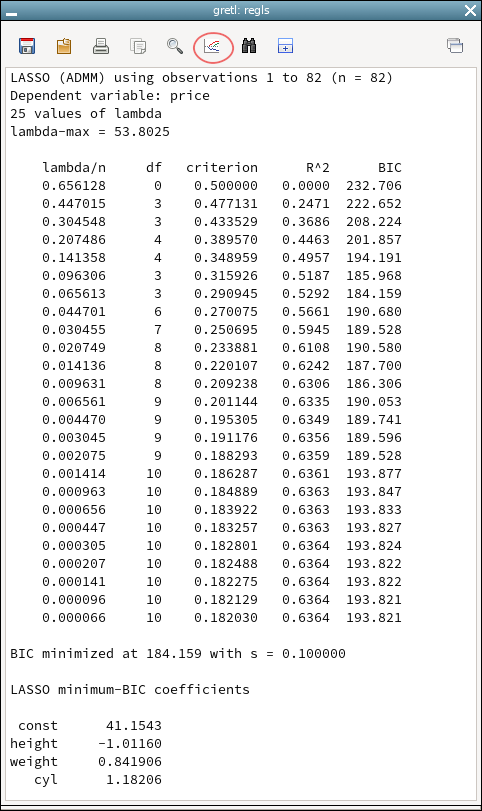
\includegraphics[scale=0.5]{regls_output}
  \end{tabular}
  \caption{\texttt{regls} dialog and output window (with Graph button circled)}
  \label{fig:regls-combo}
\end{figure}

The window that appears on clicking \textsf{OK} in the dialog box (on
the right in Figure~\ref{fig:regls-combo}) shows printed output and
offers several options via the toolbar buttons.  Most of these are
generic and should be self-explanatory. Here we'll draw attention to
the button circled in red, with tooltip ``Graph''. This is active only
when estimation has been performed with multiple $\lambda$ values. In
that case it calls up a menu with two items: ``Criterion plot'' and
``Coefficient paths''. Each of these explores an aspect of the
estimates as the regularization constraint is relaxed. In the first
case it's the optimality criterion (MSE if cross validation is
performed, BIC otherwise); in the second it's the paths of individual
coefficients.  Examples are shown in Figures~\ref{fig:mse-plot} and
\ref{fig:coeff-plot}.

\begin{figure}[htbp]
  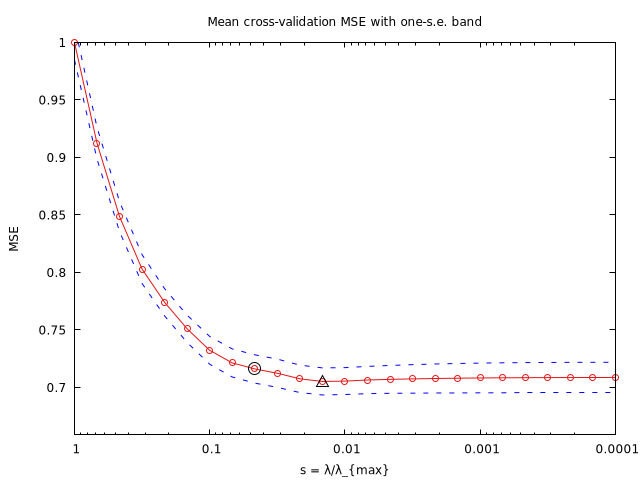
\includegraphics[scale=0.6]{mse_plot}
  \caption{MSE plot: the triangle indicates the MSE minimizer and the
    circle the ``within one standard error'' value.}
  \label{fig:mse-plot}
\end{figure}

\begin{figure}[htbp]
  \centering
  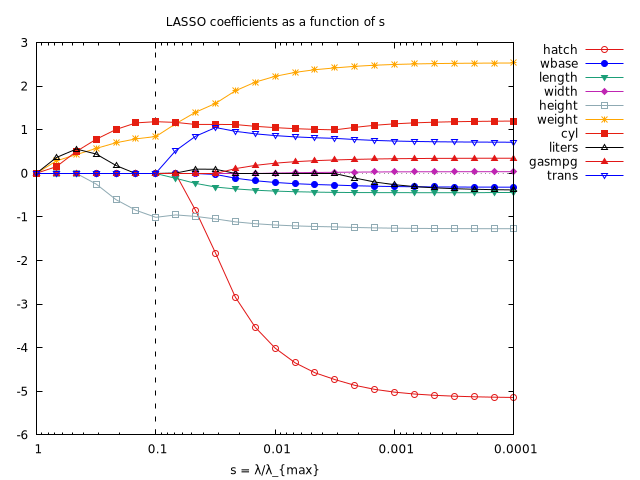
\includegraphics[scale=0.6]{coeff_plot}
  \caption{Coefficient paths}
  \label{fig:coeff-plot}
\end{figure}

To the right of the (circled) Graph button in
Figure~\ref{fig:regls-combo} is a Forecast button (binoculars
icon). If the sample was set prior to estimation so as to leave some
trailing observations for testing, this can be used to produce
out-of-sample forecast evaluation statistics, accompanied by an actual
versus predicted plot. If no out-of-sample data are available you can
still produce the evaluation statistics and plot for the within-sample
fit.

In each case the predicted values (which might be quite numerous) are
not shown, but they can be retrieved via the bundle button in the
window showing the statistics, as shown in
Figure~\ref{fig:fcast-window}. Note that in the out-of-sample case
saved predictions will not be visible via the main gretl window until
you set the sample range to include them.

%\vspace{1em}

\begin{figure}[htbp]
  \begin{center}
  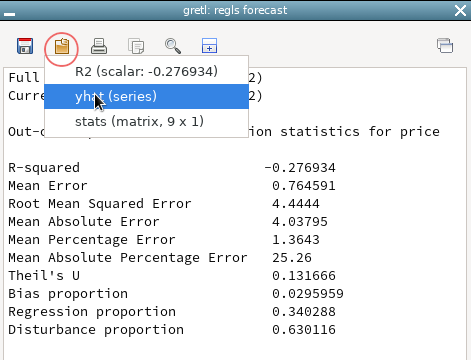
\includegraphics[scale=0.6]{fcast_series}
  \caption{Saving predictions (yhat) from the forecast output window.
    The facility for saving selected content from a bundle of results
    is also available via the bundle icon in the primary regls output
    window.}
  \label{fig:fcast-window}
  \end{center}
\end{figure}

\clearpage

\section{Reference: public functions}
\label{sec:funcref}

\begin{funcdoc}
\begin{verbatim}
bundle regls (series y, list X, bundle parms)
\end{verbatim}
  Performs LASSO, Ridge or Elastic net estimation given the dependent
  variable \texttt{y}, the regressors \texttt{X}, and options in
  \texttt{parms}. Returns a bundle containing the
  results. Table~\ref{tab:regls-parms} lists the parameters that can be
  passed via the \texttt{parms} argument.
\end{funcdoc}

\begin{table}[htbp]
  \centering
  \begin{tabular}{lll}
    \texttt{lfrac} & scalar or vector & $\lambda$-fraction(s) \\
    \texttt{nlambda} & integer & number of automatic $\lambda$s \\
    \texttt{stdize} & 0/1, default 1 & standardize the data \\
    \texttt{ridge} & 0/1, default 0 & do Ridge regression \\
    \texttt{lambda\_scale} & 0, 1 or 2, default 1 & see Section~\ref{sec:ridge} \\
    \texttt{verbosity} & 0, 1, 2 or 3, default 1 & printing of output\\
    \texttt{xvalidate} & 0/1, default 0 & do cross validation\\
    \texttt{nfolds} & optional integer $>1$, default 10 & number of
                                                          folds \\
    \texttt{randfolds} & 0/1, default 0 & use random folds\\
    \texttt{use\_1se} & 0/1, default 0 & see Section~\ref{sec:xvalid} \\
    \texttt{seed} & optional integer & controls random folds\\
    \texttt{single\_b} & 0/1, default 0 & see Section~\ref{sec:xvalid}\\
    \texttt{no\_mpi} & 0/1, default 0 & see Section~\ref{sec:speed}\\
    \texttt{admmctrl} & optional control vector & see
                                                  Section~\ref{sec:add-controls} \\
    \texttt{ccd} & 0/1, default 0 & see section~\ref{sec:ccd} \\
    \texttt{ccd\_toler} & positive scalar, default $10^{-7}$ & see
                                                               Section~\ref{sec:ccd}\\
    \texttt{alpha} & $0 \leq \alpha \leq 1$ (default 1) & see
                                                               Section~\ref{sec:elnet}
  \end{tabular}
  \caption{Summary of parameters for the \texttt{regls} function}
  \label{tab:regls-parms}
\end{table}

\begin{funcdoc}
\begin{verbatim}
matrix lambda_sequence (scalar lmax, int K, scalar eps[0.0001])
\end{verbatim}
  Produces a column vector holding a logarithmic sequence of
  \texttt{K} values running from \texttt{lmax} to \texttt{eps}. It is
  required that $0 < \mbox{\texttt{lmax}} \le 1$ and
  $0 \le \mbox{\texttt{eps}} < \mbox{\texttt{lmax}}$. In context such
  values are interpreted as instances of $s = \lambda/\lambda_{\max}$.
\end{funcdoc}

%%\clearpage

\begin{funcdoc}
\begin{verbatim}
matrix regls_get_stats (const numeric y, const numeric yhat)
\end{verbatim}
  The arguments \texttt{y} and \texttt{yhat} must be either series or
  vectors (and both of the same type).  Returns a 2-vector
  holding MSE = $\sum(y - \hat{y})^2/n$ and
  $R^2 = 1 - \sum(y - \hat{y})^2/\sum(y - \bar{y})^2$.
\end{funcdoc}

\begin{funcdoc}
\begin{verbatim}
scalar regls_pc_correct (const numeric y, const numeric yhat)
\end{verbatim}
  The arguments \texttt{y} and \texttt{yhat} must be either series or
  vectors (and both of the same type).  Returns the percentage
  of cases in which \texttt{yhat} rounded to the nearest integer
  equals \texttt{y}. Useful only when \texttt{y} is integer-valued.
\end{funcdoc}

\begin{funcdoc}
\begin{verbatim}
matrix regls_foldvec (int nobs, int nf)
\end{verbatim}
  Returns a column vector of length \texttt{nobs} in which \texttt{nf}
  successive blocks of length \texttt{nobs}/\texttt{nf} take on the
  values 1, 2,\dots, \texttt{nf}, respectively. Useful only for
  composing a \texttt{folds} vector than can be passed to
  \textsf{glmnet} for comparison with gretl when consecutive folds are
  used in cross validation.
\end{funcdoc}

\begin{funcdoc}
\begin{verbatim}
void regls_multiprint (const bundle b, const numeric y, const numeric X)
\end{verbatim}
  The bundle argument \texttt{b} should be obtained via \texttt{regls}
  or \texttt{mregls} estimation with several \texttt{lfrac} values, as
  in Section~\ref{sec:simple-search} or \ref{sec:xvalid} above. The
  arguments \texttt{y} and \texttt{X} should be the same as those
  passed to \texttt{regls} (\texttt{y} a series, \texttt{X} a list) or
  \texttt{mregls} (\texttt{y} an $n$-vector, \texttt{X} an
  $n \times k$ matrix). This function prints a summary table showing
  $R^2$, the sum of absolute values of the coefficients, and df (the
  number of non-zero coefficients) associated with each value of
  $\lambda$. Usage is illustrated in the example script
  \texttt{lambda\_sequence.inp}, which is reproduced in part in
  Listing~\ref{script:lamseq}.
\end{funcdoc}

\begin{funcdoc}
\begin{verbatim}
void regls_coeff_plot (const bundle b, const list L[null], string fname[null])
\end{verbatim}
  Produces a plot showing the paths of coefficient estimates as the
  regularization constraint is progressively relaxed. The bundle
  argument should be obtained via \texttt{regls} estimation with
  multiple \texttt{lfrac} values, as in
  Section~\ref{sec:simple-search} or \ref{sec:xvalid} above.

  The optional list argument can be used to select for tracking a
  subset of the \texttt{X} list argument to \texttt{regls}.  This is
  recommended if the model includes a large number of independent
  variables; the plot becomes unreadable if more than 20 or so
  coefficients are shown.

  The optional \texttt{fname} argument can be used to direct output to
  file, as described in the documentation for gretl's \texttt{gnuplot}
  command. By default the plot is shown on screen.

  See also \texttt{mregls\_coeff\_plot} below.
\end{funcdoc}

\begin{funcdoc}
\begin{verbatim}
void regls_criterion_plot (const bundle b, string fname[null])
\end{verbatim}
  Produces a plot showing the path of the penalized fit criterion (BIC
  if cross validation is not performed, otherwise the MSE obtained via
  cross validation) as the regularization constraint is progressively
  relaxed. The bundle argument should be obtained via \texttt{regls}
  of \texttt{mregls} estimation with multiple \texttt{lfrac} values,
  as in Section~\ref{sec:simple-search} or \ref{sec:xvalid} above.
  The optional \texttt{fname} argument can be used to direct output to
  file, as described in the documentation for gretl's \texttt{gnuplot}
  command. By default the plot is shown on screen.
\end{funcdoc}

\begin{funcdoc}
\begin{verbatim}
numeric regls_pred (const bundle b, const list X)
\end{verbatim}
  A convenience function for producing predicted values. The bundle
  argument should be obtained via \texttt{regls}. The argument
  \texttt{X} must be the same list of series that was passed to
  \texttt{regls} (although of course the sample range may differ), and
  the return value is by default a series. This function automatically
  handles the presence or absence of an estimated intercept, as well
  as selection of a specific coefficient vector when estimation has
  been performed for multiple values of the regularization parameter.
  See also \texttt{mregls\_pred} below. See Section~\ref{sec:predict}
  for details.
\end{funcdoc}

\begin{funcdoc}
\begin{verbatim}
bundle mregls (const matrix y, const matrix X, bundle parms)
\end{verbatim}
  This function works like \texttt{regls()}, except that \texttt{y} is
  a column vector of length $n$ and \texttt{X} is an $n \times k$
  matrix. The options accepted in \texttt{parms} are as described in
  Table~\ref{tab:regls-parms} above. Consistent with the different
  input types, one element in the output bundle also differs in type:
  in \texttt{regls} output \texttt{nzX} is a list of series while in
  \texttt{mregls} output it is a selection vector, picking out the
  columns of the \texttt{X} matrix that have non-zero coefficients.
\end{funcdoc}

\begin{funcdoc}
\begin{verbatim}
matrix mregls_pred (const bundle b, const matrix X)
\end{verbatim}
  Companion to \texttt{regls\_pred}, for a bundle obtained via
  \texttt{mregls}. The matrix \texttt{X} must have the same number of
  columns as that passed to \texttt{mregls}. The return value is by
  default a column vector of length equal to the row dimension of
  \texttt{X}.  This function automatically handles the presence or
  absence of an estimated intercept, as well as selection of a
  specific coefficient vector when estimation has been performed for
  multiple values of the regularization parameter. See
  Section~\ref{sec:predict} for details.
\end{funcdoc}

\begin{funcdoc}
\begin{verbatim}
void mregls_coeff_plot (const bundle b, const matrix sel[null], string fname[null])
\end{verbatim}
  Works just like \texttt{regls\_coeff\_plot} (see above) except that
  this variant is for use after \texttt{mregls} estimation. The
  optional selection of coefficients to be tracked works via a
  selection (row) vector. The elements of this vector should be column
  indices pertaining to the \texttt{X} matrix argument to
  \texttt{mregls}.
\end{funcdoc}

\begin{funcdoc}
\begin{verbatim}
series glmnet_pred (matrix *Rb, list X)
\end{verbatim}
  Convenience function for handling results retrieved by gretl from
  \textsf{glmnet}. On entry \texttt{Rb} should hold the full
  coefficient vector (including any zeros) and \texttt{X} the full
  list of candidate regressors, and the return value is the result of
  \texttt{lincomb(X, Rb)}. On exit \texttt{Rb} holds only the non-zero
  coefficients, with row-names added based on the \texttt{X}
  list. This is then comparable with gretl's \texttt{nzb}.
\end{funcdoc}

\begin{funcdoc}
\begin{verbatim}
void glmnet_multiprint (const matrix RB, const matrix Rlam,
                        const bundle b, const series y, list X)
\end{verbatim}
  Convenience function for facilitating comparison of results when the
  same regularization task has been performed in gretl using
  \texttt{regls} and in \textsf{R} using \texttt{glmnet}. The output
  is like that of \texttt{regls\_multiprint}.  The matrices
  \texttt{RB} and \texttt{Rlam} should be obtained from the object
  returned by \texttt{glmnet()}; \texttt{b} should be the bundle
  returned by \texttt{regls}.  Usage is illustrated in
  Listing~\ref{script:lamseq}.
\end{funcdoc}

\section{Change log}
\label{sec:changes}

2024-04-29: Add specific prediction and plotting functions for use
with \texttt{mregls}; implement fixes for the unlikely case where none
of the candidate regressors are effective predictors of the dependent
variable; make plots more robust; add descriptive labels to the
included murder-rates dataset; expand and update the documentation.\\[4pt]
2023-05-20: Add support for matrix input via the \texttt{mregls}
function; simplify the signature of \texttt{regls\_multiprint};
add function \texttt{glmnet\_multiprint}.\\[4pt]
2022-10-02: Enhancements for regls plots; document GUI usage; update
an internal function signature to comply with gretl's
new ``const inheritance'' policy.\\[4pt]
2022-08-05: fix breakage for single-lambda case.\\[4pt]
2022-06-03: update URL; revise fragile list-saving code;
allow ``lambda'' as alternative to ``lfrac'' on input.\\[4pt]
2021-04-17: fix bug with Ridge verbose printout, and replace some
tables with figures in the doc for ease of comprehension
of comparative experiments.\\[4pt]
2021-01-29: support a higher verbosity level for GUI use;
improve printout for LASS0 coefficients, when applicable.\\[4pt]
2020-10-09: initial release.

\begin{script}
  \caption{LASSO with lambda sequence}
  \label{script:lamseq}
\begin{scode}
set verbose off
include regls.gfn

open murder.gdt --quiet --frompkg=regls

# all available predictors w. no missing values
list X = population..LemasPctOfficDrugUn

smpl 1 800
printf "Sample range %d to %d\n", $t1, $t2

bundle parms = _(nlambda = 8, verbosity = 0)

bundle b1 = regls(murdPerPop, X, parms)
printf "\ngretl (ADMM):\n"
regls_multiprint(b1, murdPerPop, X)

parms.ccd = 1
bundle b2 = regls(murdPerPop, X, parms)
printf "\ngretl (CCD):\n"
regls_multiprint(b2, murdPerPop, X)

# STOP here if R + glmnet is not available
# quit

# R::glmnet
list LL = murdPerPop X
foreign language=R --send-data=LL
  library(glmnet)
  x <- as.matrix(gretldata[,2:ncol(gretldata)])
  y <- as.matrix(gretldata[,1])
  m <- glmnet(x, y, family = "gaussian", alpha = 1, nlambda = 8,
    standardize = T, intercept = T)
  Rb <- as.matrix(coef(m))
  gretl.export(Rb)
  Rlam = as.matrix(m$lambda)
  gretl.export(Rlam)
end foreign

matrix Rb = mread("Rb.mat", 1)
matrix Rlam = mread("Rlam.mat", 1)
printf "\nglmnet:\n"
glmnet_multiprint(Rb, Rlam, b2, murdPerPop, X)
\end{scode}
\end{script}

\bibliographystyle{gretl}
\bibliography{gretl}

\clearpage
\startappendices

\myappendix{Comparison of algorithms}
\label{app:ccd}

This appendix reports some experiments designed to gauge the accuracy
and speed of the Cyclical Coordinate Descent (CCD) algorithm as
compared to the default algorithms in \textsf{regls}---ADMM for LASSO
and SVD for Ridge.

\subsection{Design of experiments}

The general design of our experiments is as follows. For some selected
dataset and sample range we compute the values of the minimized
objective function (LASSO or Ridge) for a sequence of $\lambda$
values. In each test we compare two optimization methods---call them A
and B---taking A as the baseline and exploring how the difference in
results between the methods behaves as we tighten the convergence
tolerance for method B. We assume that for the iterative methods ADMM
and CCD, tightening the tolerance (within reason) will produce more
accurate results, or at least will not produce less accurate
results. Therefore, if the difference diminishes as tolerance is
tightened for B we can infer that A was more accurate at the initial
tolerance level.

We measure the difference between sets of results via Euclidean
distance.\footnote{We also tried Mean Absolute Deviation but this did
  not seem to contribute additional information.}  To gauge the
trade-off between accuracy and speed we also record the execution time
for method B divided by that for A.

In the experiments reported below we used the murder rates dataset
(\texttt{murder.gdt}) supplied with the \texttt{regls} package, with
\texttt{murdPerPop} as dependent variable and 101
regressors.\footnote{This dataset was referenced by Ryan Tibshirani in
  the LASSO context; see
  \url{https://www.stat.cmu.edu/~ryantibs/datamining/lectures/17-modr2.pdf}.}
The $\lambda$ sequence was of length 20. In the LASSO tests we used
the first 800 observations and in the Ridge tests the first 1500 (to
make the test take longer and improve the resolution of the
timer). We're aware that the results we show are liable to be data-
and model-dependent and we offer some comments on this in the
concluding section.

\subsection{Ridge: SVD and CCD}

The Ridge problem has an analytical solution and \textsf{regls}
implements this using Singular Value Decomposition, which is generally
regarded as the gold standard for accuracy in digital
computation. Results obtained via SVD can therefore be used as a
benchmark against which to assess the accuracy of the solution
provided by CCD.

Figure~\ref{fig:ccd-svd} shows our findings. The distance between the
two sets of results declines monotonically as the CCD tolerance is
tightened, as one would expect. At its default tolerance of $10^{-7}$
CCD is faster than SVD (in this example by about 30 percent), but it
takes longer than SVD if one wants the extra accuracy associated with
a tolerance of $10^{-9}$ or less. Note, however, that there seems to
be little point in reducing the CCD tolerance below $10^{-9}$.

%% Ridge: CCD and SVD, using \texttt{ridge\_crit\_native.inp}
\begin{figure}[htbp]
\begin{center}
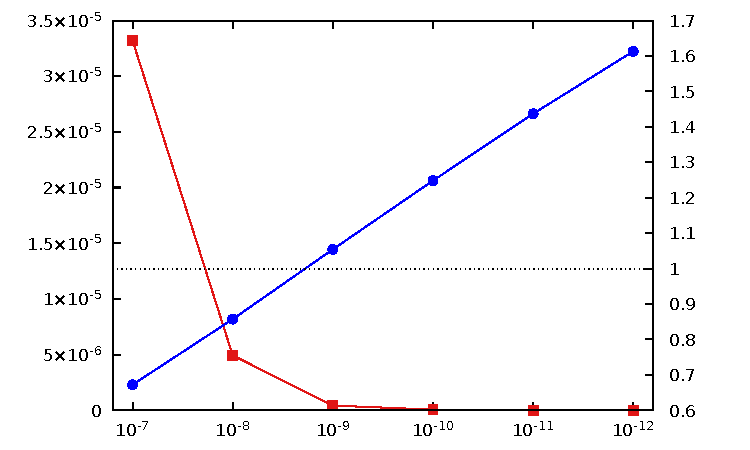
\includegraphics[scale=0.9]{ccd_svd.pdf}
\caption{Ridge regression: CCD performance relative to SVD
  baseline. CCD tolerance on $x$-axis, Euclidean distance between
  estimates in red (left) and relative execution time in blue
  (right).}
\label{fig:ccd-svd}
\end{center}
\end{figure}

\subsection{LASSO: ADMM and CCD}

LASSO is trickier than Ridge in that there's no analytical solution to
serve as a natural benchmark. In this case we take ADMM (at its
default tolerance in \textsf{regls}) as baseline---without assuming
its results are ``correct''---and see what happens.

Figure~\ref{fig:ccd-admm} shows monotonic decline in difference of
results as the CCD tolerance is tightened from $10^{-7}$ to
$10^{-10}$, at which point the results become practically
indistinguishable. We interpret this to mean that ADMM at its default
settings produces results that can be taken as ``correct'' for
practical purposes.

Notice that with LASSO the effect of tighter tolerance on the
execution time for CCD relative to the baseline is a good deal more
marked than in the Ridge case. When the CCD tolerance is reduced from
$10^{-7}$ to $10^{-9}$ Ridge time becomes slightly greater than SVD
time, while LASSO time becomes over twice that of ADMM.

%% LASSO: CCD and ADMM, using \texttt{lasso\_crit\_native.inp}
\begin{figure}[htbp]
\begin{center}
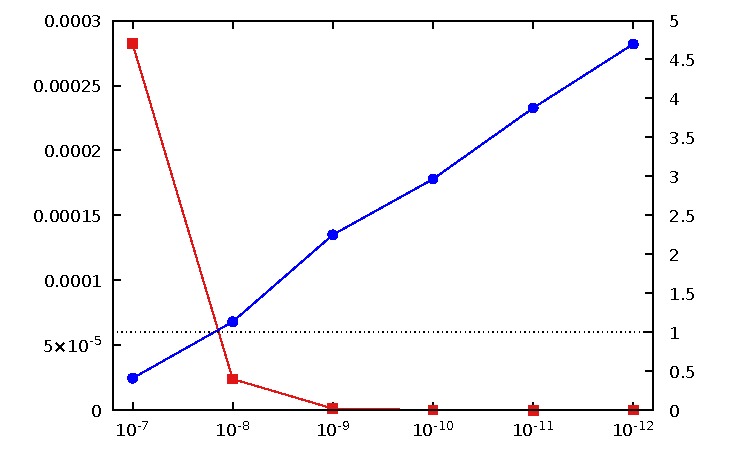
\includegraphics[scale=0.9]{ccd_admm.pdf}
\caption{LASSO estimation: CCD performance relative to ADMM
  baseline. CCD tolerance on $x$-axis, Euclidean distance between
  estimates in red (left) and relative execution time in blue
  (right).}
\label{fig:ccd-admm}
\end{center}
\end{figure}

If ADMM is more accurate than CCD at their respective default
tolerances, can we find tolerances for the former that produce similar
accuracy to the CCD default? And if so, what happens to the speed
comparison?

Figure~\ref{fig:admm-seq} shows the results of a relevant
experiment. The integers, $i$, on the $x$-axis represent progressively
slacker tolerance pairs, $(i\times 10^{-2}$, $i\times 10^{-4})$, for
ADMM.  (Note that the $i=1$ already gives values 100 times greater
than the ADMM default.) As expected, greater tolerances correspond to
shorter execution times (blue line, right-hand scale) and increasing
distance from the baseline high-accuracy ADMM results (red line,
left-hand scale).  CCD, at its default tolerance of $10^{-7}$, enters
the picture in two ways: its execution speed is by construction 1 on
the right-hand scale, while its deviation from the baseline estimates
is shown by the dotted red line.

In this example there is a range of the ADMM tolerances, comprising
$i=2$ and $i=3$, over which ADMM is both faster and more accurate than
CCD.

%% LASSO: ADMM with slacker tolerances, vs CCD
\begin{figure}[htbp]
\begin{center}
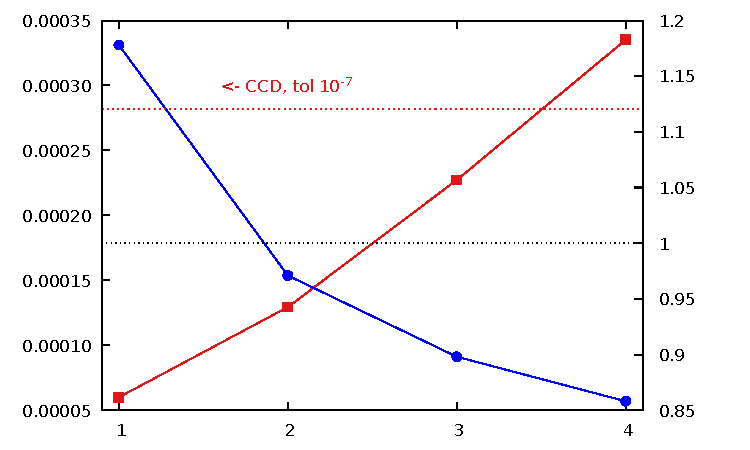
\includegraphics[scale=0.9]{admm_ccd.pdf}
\caption{LASSO estimation: ADMM performance at slacker tolerances.
  See text for explanation of $x$-axis. Euclidean distance from
  high-accuracy estimates in red (left) and time relative to CCD in
  blue (right).}
\label{fig:admm-seq}
\end{center}
\end{figure}

As noted above, such figures are likely to be data- and
model-dependent, but we conjecture that ADMM tolerances of
$(10^{-2}, 10^{-4})$ are conservative relative to CCD at tolerance
$10^{-7}$ in the sense that they are likely to deliver results of
equal accuracy to CCD or better.

\subsection{Conclusion}

The results shown above, from a single dataset, are obviously
illustrative rather than definitive. On the strength of similar tests
on other datasets we're able to say something about what is generally
applicable and what is variable.

In all of our experiments CCD at its default tolerance is faster but
less accurate than SVD for Ridge regression, and faster but less
accurate than ADMM (at its default tolerance) for LASSO. And in all
cases the accuracy of CCD can be increased (up to a point) by
reducing its tolerance.

Two things are relatively variable (apparently depending on, among other
things, the number of observations and the number of regressors,
though not in any easily predictable way).
\begin{itemize}
\item The time taken by CCD relative to the alternatives as a function
  of the CCD tolerance. In some cases (unlike the example above) CCD
  retains its speed advantage as its tolerance is reduced. While CCD
  is bound to slow down some at tighter tolerance it may still be the
  fastest method.
\item Convergence of CCD is not guaranteed. In a few LASSO trials we
  saw failure at, for example, a tolerance of $10^{-10}$, when ADMM
  had converged OK and the difference statistics seemed to show room
  for further improvement of accuracy on the part of CCD. This
  suggests that CCD is not always capable of accuracy equal to
  ADMM. It's possible that in other cases this could be reversed (ADMM
  unable to equal the accuracy of CCD), though we didn't see any such
  in our trials.
\end{itemize}

So here's our conclusion. (As a warning to the reader we have
emphasized the words that signal our remaining uncertainty!)  If you
want maximally accurate results you should use SVD for Ridge and
\textit{probably} use ADMM for LASSO. You can \textit{usually} get
equal accuracy from CCD if you tighten its tolerance far enough but
then CCD \textit{may} take longer than the alternatives. On the other
hand, if you reckon the accuracy of CCD at its default tolerance is
good enough for practical purposes you can save time by using it.
Unless, in the case of LASSO, you'd like to set the ADMM tolerances to
$(10^{-2}, 10^{-4})$, in which case you \textit{may} get somewhat more
accurate results with little difference in execution time.

To go any further we would have to assess what's ``good enough''
accuracy (for example, with out-of-sample prediction in view). Does
the extra accuracy of ADMM and SVD actually help, or is it surplus to
requirements? We have something to say about that in
\ref{app:glmnet-comp}.

\myappendix{Comparison with glmnet}
\label{app:glmnet-comp}

Given the benchmark status of \textsf{R}'s \textsf{glmnet} we have
tried to ensure that our results are very close to those from
\textsf{glmnet} unless we can demonstrate a good reason for
divergence. We comment below on reasons why results may differ in
certain respects.

\subsection{Different conventions}

It should be noted that \textsf{regls} and \textsf{glmnet} employ
different conventions in some respects. This does not affect the
comparison of reported coefficients or predicted values, but it can
make comparison of $\lambda$ values a little awkward. The LASSO
objective function and definition of $\lambda_{\max}$ used by
\textsf{regls} were stated in Section~\ref{sec:intro}, but to be fully
explicit we should say that the $X$ and $y$ in equation
(\ref{eq:lmax}) for the maximum $\lambda$ are taken to be standardized
values.

In \textsf{glmnet} the objective (in the linear Gaussian case) is
\[
   \min_{\hat{\beta}} \quad \frac{1}{2n}\,
  \sum_{i=1}^n (y_i - X_i\hat{\beta})^2 + \lambda \sum_{j=1}^k |\hat{\beta}_j|
\]
This differs from our equation (\ref{eq:obj}) in dividing the sum of
squared residuals (SSR) by $2n$ rather than 2. Since \textsf{glmnet}
is not actually using a different relative weighting of the SSR and
the sum of absolute coefficient values, it follows that their
``$\lambda$'' must be read as $n^{-1}$ times ours. Moreover, while we
take each $\lambda_i$ value to be $s_i$ times $\lambda_{\max}$ as
defined in equation (\ref{eq:lmax}), the $\lambda$ values printed by
\textsf{glmnet} are (in our notation)
\[
\lambda_i = s_i \cdot \lambda_{\max} \cdot \hat{\sigma}_y / n
\]
where $\hat{\sigma}_y$ is the ML estimate of the standard deviation of
the dependent variable. To obtain the \textsf{glmnet} $\lambda$
corresponding to a given $s$ one can do:
\begin{code}
Rlam = s * b.lmax * sdc({y}) / b.nobs
\end{code}
where \texttt{b} is a bundle obtained via \texttt{regls} on the same
data, \texttt{y} is the dependent series and \texttt{sdc(\{y\})} gives
$\hat{\sigma}_y$. The current sample range must be the same as for
\texttt{b} to get $\hat{\sigma}_y$ right, but if \textsf{glmnet} was
told \textit{not} to standardize the data then this term should be
omitted as it is assumed to be 1.

\subsection{Cross validation methodologies}

There's a substantive difference between \textsf{regls} and
\textsf{glmnet} in respect of cross validation. This applies even if
the CCD algorithm is selected in \textsf{regls}, which results in
near-identical results for LASSO or Ridge coefficients when simply
processing a sequence of $\lambda$ values.

In \textsf{regls} cross validation, the entire training dataset is
standardized at the outset, then each fold gets its share of the
standardized data. The maximum $\lambda$ is also determined using the
full training set and the same $\lambda$ sequence is used for each
fold. In \textsf{glmnet}, by contrast, both standardization and
calculation of the $\lambda$ sequence are done per fold. For example,
suppose the training data are divided into 10 folds, each comprising
10 percent of the observations. Then \textsf{glmnet} both standardizes
and computes a $\lambda$ sequence using the complementary 90 percent
of the data.

\subsection{Extended test of cross validation}

The primary point of cross validation is to determine the value of a
hyperparameter (for LASSO, $\lambda$) that is likely to give best
results in genuine out-of-sample prediction. In this section we
describe some experiments designed to probe the impact (if any) of
certain differences noted above on the efficacy of out-of-sample
prediction. We are particularly interested in
\begin{itemize}
\item the methodological difference between \textsf{regls} and
  \textsf{glmnet} noted in the previous section, and
\item the ``extra accuracy'' of the ADMM algorithm, at its default
  tolerance, over CCD at its default tolerance, noted in
  \ref{app:ccd}.
\end{itemize}

As regards the methodological difference, not a great deal can be said
about this \textit{a priori}, though one thing is clear: the more
homogeneous the training data, the less details of method are going to
matter. If the statistical properties of the fold-complement samples
are very similar to those of the full training data then the locus of
standardization (training data or fold-complement) won't make much
difference. In addition, if $\lambda_{\max} = \|X'y\|_{\infty}$
doesn't differ much across the samples the locus of calculation of the
$\lambda$ sequence won't matter much either, and
$\lambda$-matching---if it is required---should be relatively
unproblematic.

That said, real-world datasets of interest are not necessarily very
homogeneous so the details \textit{could} matter. To investigate this
we ran experiment on two rather different datasets.
\begin{itemize}
\item Dataset 1: murder rates and covariates for US localities
  (\texttt{murder.gdt}, supplied with the \textsf{regls} package).
  Comprises 2215 observations on 102 variables.
\item Dataset 2: white wine quality and physico-chemical covariates.
  Comprises 4898 observations on 12 variables (78 after adding squares
  and interactions of covariates).\footnote{See
    \url{https://archive.ics.uci.edu/ml/datasets/wine+quality}.}
\end{itemize}

We ``leveraged'' the datasets by randomizing the order of the
observations at each of 2000 iterations then taking the first $N$
observations for training and the next $M$ for testing, with $N+M$
a subset of the full data available. For Dataset 1 $N=1200$ and
$M=200$, and for Dataset 2 $N=1500$, $M=500$.

The body of the test involved cross validating with 10 folds (composed
of consecutive observations since the whole dataset was randomized)
then predicting for the $M$ holdout observations using the optimal
$\lambda$ on the ``one standard error'' rule favored by
\textsf{glmnet}. This rule selects the larger of (a) the $\lambda^*$
which minimizes mean out-of-sample MSE and (b) the largest $\lambda$
that lies within $\sigma^*$ of $\lambda^*$, where $\sigma^*$ is the
standard error of the minimized mean MSE.\footnote{The mean is taken
  across the folds, weighted if necessary.} The figure of merit
calculated at each iteration was the $R^2$ for the testing data,
$1 - \sum (y-\hat{y})^2 / \sum (y-\bar{y})^2$.

This test was run (with common randomization) using three variants of
cross validation, each with its default settings: the \textsf{glmnet}
function \texttt{cv.glmnet}; \textrm{regls} using the CCD algorithm;
and \textsf{regls} using the ADMM algorithm. As mentioned above, there
are two distinct differences at play. In comparing \textsf{glmnet}
with \textsf{regls} CCD the coefficient vectors produced for given
data and given $\lambda$ are near-identical, and the relevant
difference lies in the details of the cross validation methodology. In
comparing \textsf{regls} CCD and ADMM the cross validation method is
exactly the same and the relevant difference lies in the ``excess
precision'' afforded by ADMM over CCD, at their respective default
tolerances, as discussed in \ref{app:ccd}.

%% \subsection{Dataset 1}

Statistics for out-of-sample $R^2$ from the Dataset 1 experiment are
shown in Table~\ref{tab:dset1}. In this experiment \textsf{regls} CCD
gave better out of sample prediction than \textsf{glmnet}, and ADMM
did a little better again. The first difference---due to cross
validation methodology---appears to be more substantial than the
second.

\begin{table}[htbp]
  \centering
  \begin{tabular}{rccccccc}
 & mean & s.d. & s.e.(mean) & 95\% C.I. & median & min & max \\
      glmnet & 0.4724 & 0.1518 & 0.0034 & 0.4657 - 0.4790 & 0.4881 & $-$2.6289 & 0.7044 \\
        CCD & 0.4954 & 0.1545 & 0.0035 & 0.4886 - 0.5022 & 0.5118 & $-$2.7911 & 0.6900 \\
       ADMM & 0.4984 & 0.1608 & 0.0036 & 0.4914 - 0.5055 & 0.5172 & $-$2.7831 & 0.6925 \\
  \end{tabular}
  \caption{Out of sample $R^2$, 2000 replications, Dataset 1}
  \label{tab:dset1}
\end{table}

Figure~\ref{fig:dset1} gives another angle on the comparisons,
plotting estimated kernel densities for the three
variants.\footnote{We truncated the plot on the left to focus on the
  bulk of the distributions; instances of $R^2 < 0.2$ were rare, and
  their frequency did not differ much by method.}

\begin{figure}[htbp]
  \centering
  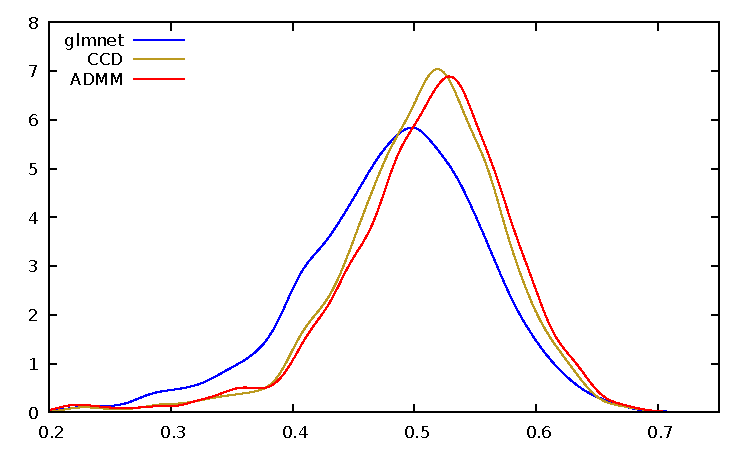
\includegraphics[scale=0.9]{murder_kd3.pdf}
  \caption{Estimated densities for out of sample $R^2$, Dataset 1}
  \label{fig:dset1}
\end{figure}

Since each method was given the same data at each iteration,
paired-difference tests for $R^2$ might be considered appropriate;
these are shown in Table~\ref{tab:paired}, along with the correlations
across the methods per iteration.

\begin{table}[htbp]
\begin{center}
  \begin{tabular}{rrr}
    & $|z|$ & $\rho$ \\[4pt]
glmnet, regls CCD & 20.6 & 0.946 \\
glmnet, regls ADMM & 21.6 & 0.942 \\
regls CCD, regls ADMM & 8.4 & 0.996 \\
  \end{tabular}
  \caption{Paired-difference tests and correlations, out of sample $R^2$}
  \label{tab:paired}
\end{center}
\end{table}

From this point of view all the differences are strongly statistically
significant, though the advantage of ADMM over CCD might not be
considered of much practical importance.

%% \subsection{Dataset 2}

Table~\ref{tab:dset2} shows out-of-sample $R^2$ statistics for Dataset
2. Again ADMM has the highest mean and median, and regls CCD does
better than glmnet on these criteria, but here the differences are
relatively small. Kernel densities are shown in
Figure~\ref{fig:dset2}. The displacement of the distribution between
methods, in the same direction as for Dataset 1, is
appreciable\footnote{And statistically significant: paired-difference
  $|z| = 19.9$ for glmnet vs CCD and $5.8$ for CCD vs ADMM.} but
maybe not large enough to be of practical importance.

\begin{table}[htbp]
  \centering
  \begin{tabular}{rccccccc}
 & mean & s.d. & s.e.(mean) & 95\% C.I. & median & min & max \\
      glmnet & 0.2735 & 0.0518 & 0.0012 & 0.2712 - 0.2758 & 0.2775 & $-$0.5072 & 0.3994 \\
         CCD & 0.2763 & 0.0523 & 0.0012 & 0.2740 - 0.2786 & 0.2803 & $-$0.5072 & 0.3994 \\
        ADMM & 0.2774 & 0.0558 & 0.0012 & 0.2750 - 0.2799 & 0.2826 & $-$0.5260 & 0.4029 \\
  \end{tabular}
  \caption{Out of sample $R^2$, 2000 replications, Dataset 2}
  \label{tab:dset2}
\end{table}

\begin{figure}[htbp]
  \centering
  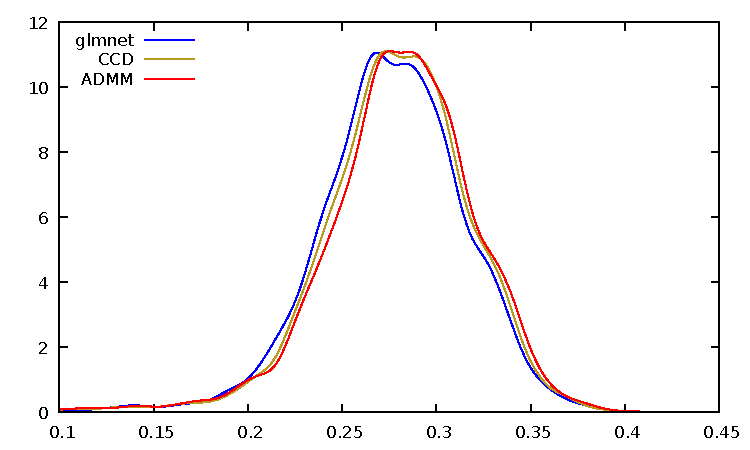
\includegraphics[scale=0.9]{wine_kd3.pdf}
  \caption{Estimated densities for out of sample $R^2$, Dataset 2}
  \label{fig:dset2}
\end{figure}

\subsection{Dataset heterogeneity}

Can we account for the difference in results between Dataset 1 and
Dataset 2 by reference to the relative heterogeneity of the data?
It's not obvious how such heterogeneity can best be measured, but we
tried a rough and ready heuristic with focus on the dependent
variable: how much do its sample statistics vary across the
fold-complement samples, relative to the full training data?

We calculated two statistics, $H_\mu$ and $H_\sigma$, for each
dataset, using the randomize-and-subset procedure described above.  At
each of 2000 iterations, $i$, we summed the absolute proportional
deviations of the fold-complement sample means,
$\bar{y}_{ij},\, j=1,2,\dots,10$, from the sample mean for the
training data, $\bar{y}_i$. We then took the mean of these values
across the iterations:
\[
  H_\mu = \frac{1}{2000} \sum_{i=1}^{2000} \sum_{j=1}^{10} |\bar{y}_{ij} - \bar{y}_i|/|\bar{y}_i|
\]
$H_\sigma$ was calculated in an exactly analogous way, with the sample
standard deviations in place of the means.  The values of these
measures for the datasets were
\begin{center}
  \begin{tabular}{lcc}
    & $H_\mu$ & $H_\sigma$ \\
    Dataset 1 & 0.12059 & 0.15032 \\
    Dataset 2 & 0.01039 & 0.05089
  \end{tabular}
\end{center}
Thus it appears that---on this crude measure at least---Dataset 2 is a
good deal more homogeneous than Dataset 1. This is consistent with the
observation that differences in out-of-sample performance attributable
to differences in the algorithms were much smaller for Dataset 2.

\subsection{Conclusion}

It's risky to conclude much on the strength of just two
datasets---even when leveraged by randomization and subsetting. But it
does seem that standardization at the level of the full training data,
and employment of a single $\lambda$ sequence---derived from the full
training data and applied for all folds---may be conducive to best
out-of-sample prediction. It also seems that the extra precision of
ADMM at its default setting is helpful for out-of-sample prediction,
though this effect is relatively small and may or may not be
considered worthwhile.

\subsection{Example script}

An example script used with Dataset 1 is shown on the following page.
This instance produces results for \textsf{regls} CCD and
\textsf{glmnet}. Results for \textsf{regls} ADMM can be obtained by
omitting the \texttt{ccd} setting in the \texttt{parms} bundle.  To
explore a different randomization one could comment out the
\texttt{set seed} line, in which case the seed for the random number
generator will be set from the clock on start-up.

\clearpage

\begin{script}
  \caption{Monte Carlo script for out-of-sample prediction}
  \label{script:mc}
\begin{scode}
set verbose off
set R_lib on
set R_functions on
include regls.gfn
open murder.gdt --quiet --frompkg=regls

# obtain results for regls CCD and cv.glmnet

foreign language=R
  lasso_R <- function(x,y,f,nl) {
    if (! "glmnet" %in% (.packages())) {
       library(glmnet)
    }
    m <- cv.glmnet(x, y, foldid = f, family = "gaussian", alpha = 1,
      nlambda = nl, standardize = T, intercept = T)
    Rb <- as.matrix(coef(m$glmnet.fit, s = m$lambda.1se))
  }
end foreign

# all available predictors without missing values
list X = population..LemasPctOfficDrugUn
list X0 = const X # for glmnet prediction

bundle parms = _(nlambda=50, verbosity=0, ccd=1, xvalidate=1)
parms.nfolds = 10
parms.use_1se = 1

# for glmnet
matrix foldvec = regls_foldvec(1200, 10)

set seed 997361
K = 2000
matrix OSR2 = zeros(K,2)

loop i=1..K --quiet
   smpl full
   series sorter = uniform()
   dataset sortby sorter

   smpl 1 1200 # training data
   bundle b = regls(murdPerPop, X, parms)
   matrix Rb = R.lasso_R({X}, {murdPerPop}, foldvec, 50)

   smpl 1201 1400 # testing data
   series pred = lincomb(b.nzX, b.nzb)
   m = regls_get_stats(murdPerPop, pred)
   OSR2[i,1] = m[2]
   series Rpred = lincomb(X0, Rb)
   m = regls_get_stats(murdPerPop, Rpred)
   OSR2[i,2] = m[2]
endloop

mwrite(OSR2, "murder_ccd.mat")
\end{scode}
  \end{script}

\end{document}
